\documentclass{article}
\usepackage[utf8]{inputenc}
\usepackage{xcolor}
\usepackage{url}
\usepackage[nottoc]{tocbibind}
\usepackage{graphicx}
\usepackage[bottom]{footmisc}
\usepackage{float}


\title{CSCE 479/879 Homework 2:
Sentiment Analysis with Sequential Models}
\author{Kantilata Thapa\\
Puranjit Singh\\
Shubham Bery\\
Shiva Paudel}
%\date{January 2021}

\begin{document}

\maketitle

\begin{abstract}
    For this homework, our team developed deep learning models to perform sentiment analysis on the IMDB dataset. This dataset has a total of 50000 movie reviews that have been labeled with “positive” and “negative” sentiment class labels. We came up with two architectures based on LSTM cells and attention mechanism. The main focus was to observe the effect of various
hyper-parameters on the model's capability to best generalize the unseen data.
The maximum validation accuracy obtained by model in the first architecture was 0.8708 with a 95\% confidence interval of (0.1221, 0.1369)
for the generalization error. This was also the overall best model among
both architectures. For the second model architecture, the maximum validation accuracy observed was 0.8688 with a 95\% confidence interval of
(0.1206, 0.1348) for the generalization error. The difference between the
two model architectures is that the second model architecture has deeper network making use of extra convolution and dropout layers.
This did not increase the validation accuracy but helped to decrease the overfitting problem as
compared to the first model architecture.

\end{abstract}

\section{Introduction}
\label{sec:intro}

Deep learning uses various algorithms in a progressive chain of events which can solve complex problems and allows us to tackle massive amount of data, accurately with minimal human interaction. In natural language processing, sentiment analysis plays important role to determine whether language reflects a positive, negative or neutral sentiment. The main objective of this homework was to build and train sequential neural networks to classify text as either negative or a positive review. Two different types of model architecture were developed, one with LSTM recurrent neural network and other with more deeper network making use of extra convolution and dropout layers. In both model architecture attention mechanism was used, and performance of the model was evaluated with change of hyperparameters such as learning rate, k-fold cross validation , epochs, L1-L2 regularization and learning rate. In second model architecture, LSTM cells,dropout and dense layers were used additionally for hyperparameter tuning. The maximum validation accuracy given by model architecture 1 was 0.87 and lowest validation loss was 0.28. Similarly, we obtained highest validation accuracy of 0.869 and lowest validation loss of 0.30 with model architecture 2 .Interval estimates were also calculated and constructed for the generalization error of all sets of hyperparameters in order to select the best performing models in both architecture. 



\section{Problem Description}

 We worked on IMDB datasets for this homework. The main goal of this learning problem was to develop sequential neural network models to perform sentiment analysis on the datasets and predict either they will give positive or negative reviews. We made use of Long-Short Term Memory (LSTM) recurrent neural networks and attention mechanism for model building. This can be fruitful for businesses to analyze customer reviews and improve customer services based on reviews analysis done by the model.

\subsection{IMDB Dataset}
 The IMDB movie reviews dataset is a binary sentiment analysis dataset which consists of 50000 reviews from the internet movie database separated into positive or negative review categories. The dataset contains an equal number of positive and negative reviews. The reviews are preprocessed, and each review is encoded as a list of word indexes (integer). The dataset consists of 25000 highly polarized movie reviews in both training and testing dataset \cite{TFData}.

\section{Approaches}

In order to solve sentiment analysis  problem for the classification of IMDB review datasets ,we developed two model architectures . This section describes a detail description of those model architecture and all the pre-processing is done inside the developed networks.   
\begin{figure}[H]
    \centering
    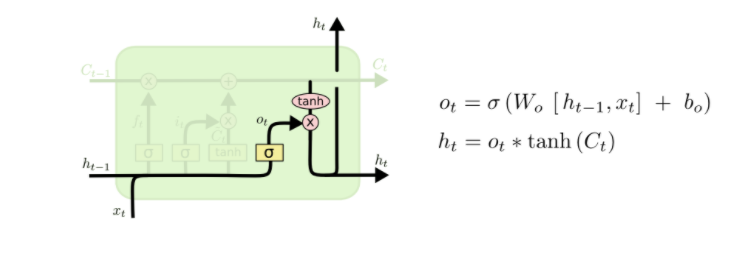
\includegraphics[width=\textwidth]{LSTM.PNG}
    \caption{LSTMcell by \cite{LSTM}}
    \label{fig:Lstm}
\end{figure}
LSTM (Long Short Term Memory) are the most powerful and well known subset of artificial neural network which  are designed to recognize patterns in sequences of data like numerical time series, text, handwriting and the spoken words. They are capable of learning order dependence in sequence prediction problem. The reason LSTM are used is they enable RNN (Recurrent Neural Networks) to remember inputs over a long period of time and solve a problem of vanishing and exploding gradients \cite{yu2019review}. LSTMs have three gates namely input, forget and output gate which determine weather or not to let new input in, delete the information or let it impact the output at the current timestep.  


\subsection{Model Architecture 1}

In the first model architecture, we implemented LSTM recurrent neural network with one dense layer in the end. We applied attention mechanism in this model. Figure \ref{fig:compute1} shows the model architecture 1, initially IMDB dataset were loaded and splitted into training set and validation set. Then text vectorization layer was applied which setup preprocessor to turn word into integers. Following embedding layer transforms each integer into a relatively small, dense vector. Given the tendecy of RNN to lose revelant information in the initial time step, an attention mechanism can be developed to use all the encoded steps of the RNN and then use a weighted sum of these encoded steps to predict. We implemeted a simplest Luong based attention mechanism on two Conv1D layes as shown in \ref{fig:compute1} \cite{luong2015effective}. Finally, the logits are passed through a dense layer with RELU activtion function to predict the sentiment of the review. \par
With this implemented model we plan to analyse the performance of different sets of hyperparameters. We have chosen k-fold cross validation, epochs, L1 and L2 regularize,  and learning rate as the parameter under study. While we go on training the model with different set of hyperparameters, we updated them with best performance and expected to get better results at the end of  the trial runs.

\begin{figure}[H]
    \centering
    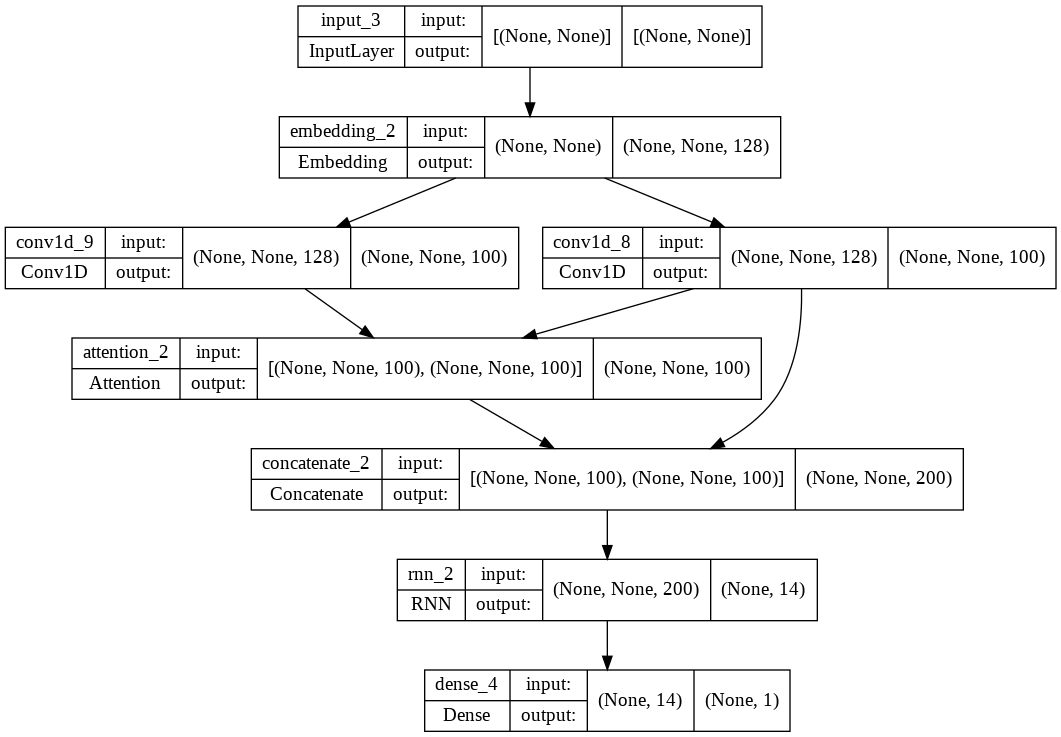
\includegraphics[width=\textwidth]{Model1.PNG}
    \caption{Model Architecture 1 with various trail run}
    \label{fig:compute1}
\end{figure}

\subsection{Model Architecture 2}
In the second model architecture, we implemented the same LSTM recurrent neural network in a single fully connected layer with two dense layers at the end. We  applied attention mechanism in this model as well. Also, we included a few more convolutional layers in this architecture as compared to former with some pooling layers. In this model, we analyzed output performance of various hyperparameters, namely k-fold cross validation, epochs, learning rate, dropout and LSTM cells. We tuned and tweaked these hyperparamter values in order to compare and check on how they affect the performance of our proposed model.\\

The model architecture 2 is described in the given figure \ref{fig:compute2} which depicts the model is deeper as compared to former and includes more convolutional and dense layers in it. Initially, IMDB dataset were loaded and splitted into training and validation set separately. The main intuition behind using more convolutional and dense layers including attention mechanism in this architecture is to check on how well the model performs by comparing the validation accuracy and loss values after the model trains on our input IMDB datasets. 

\begin{figure}[H]
    \centering
    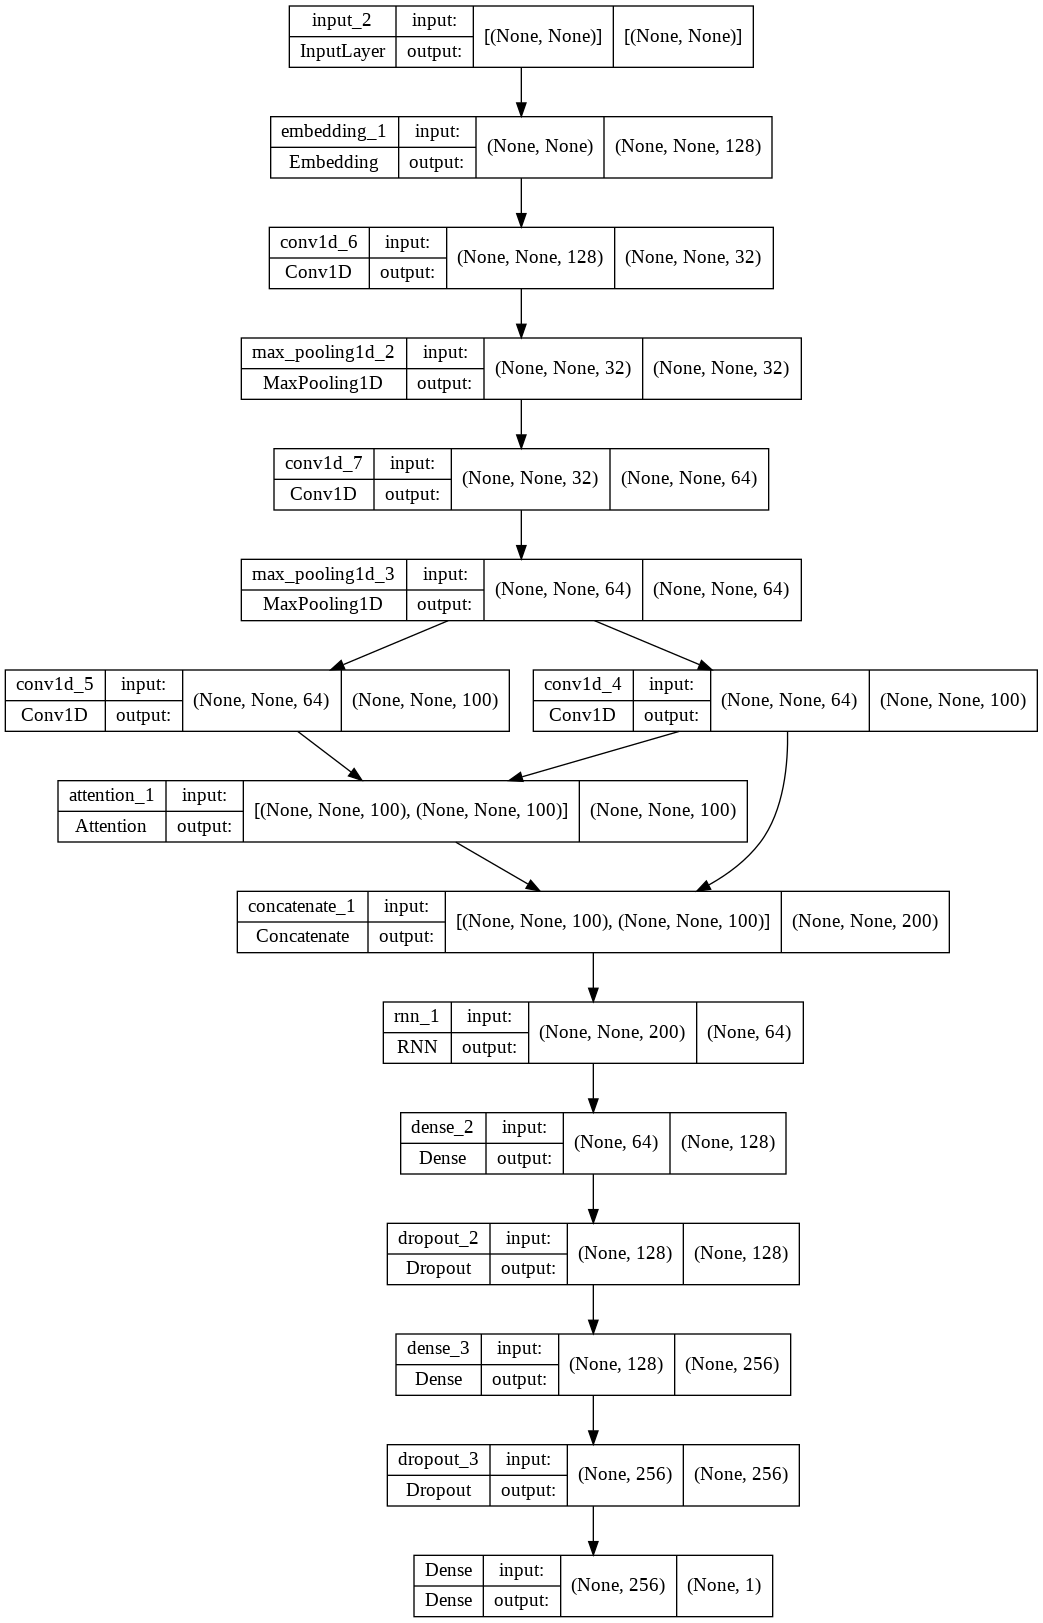
\includegraphics[width=0.9\textwidth]{Model 2.png}
    \caption{Model Architecture 2 with various trail run}
    \label{fig:compute2}
\end{figure}

%%%%%%%%%%%%%%%%%%%%%%%%%%%%%%%%%%%%%%%%%%%%%%%%%%%%%%%%%%%%%%%
%
% Welcome to Overleaf --- just edit your LaTeX on the left,
% and we'll compile it for you on the right. If you open the
% 'Share' menu, you can invite other users to edit at the same
% time. See www.overleaf.com/learn for more info. Enjoy!
%
%%%%%%%%%%%%%%%%%%%%%%%%%%%%%%%%%%%%%%%%%%%%%%%%%%%%%%%%%%%%%%%

\section{Experimental Setup}
This section provides a overview of experimental setup that were conducted  during architecture model 1 and architecture model 2. 
At first , the IMDB datasets for the classification task was imported form TensorFlow datasets and splitted into  training set –50\% and validation set-50\%. For both model architecture data import process and splitting process into training and validation sets was done in a similar manner. A GPU environment helped speed up the process of model fitting.

\subsection{Model Architecture 1}
The first model architecture starts with the pre-processing of word input sequences. After defining  the network, the model is complied and trained with different sets of hyperparameter tuning. The different hyperparameters defined/used in the architecture 1 are K-fold cross-validation, epochs, regularizer used and learning rates. Different sets of these hyperparamter values were used while training our model and the values used are described in a detail way in the following table.\\

\begin{tabular}[H]{ | p{0.5cm}||p{2cm}||p{2cm}||p{2cm}||p{2.25cm}|}
\hline

 \multicolumn{5}{|c|}{ Table 1:Summary of hyperparameters used for variants in Model Architecture 1 } \\
 \hline
 Sr. No. & K-fold cross-validation & Epochs & Regularizer & Learning rate\\
 \hline
 1 & 2  & 4  & None & 0.001  \\
 2 & 4 & 4  & None & 0.001  \\
 3 & 4 & 2 & None & 0.001  \\
 4 & 4 & 1& None & 0.001  \\
 5 & 4 & 2 & `L2'& 0.001  \\
 6 & 2 & 2 & `L1'& 0.001 \\
 7 & 2 & 2 & `L2'& 0.01 \\
 8 & 2 & 2 & `L2'& 0.0001 \\
 \hline

\end{tabular}

\subsection{Model Architecture 2}

The second model architecture performs the same pre-processing of word input sequences as in the former architecture. After defining  the network, the model is complied and trained with different sets of hyperparameter tuning. The different hyperparameters defined/used in the architecture 2 are K-fold cross-validation, epochs, LSTM cell vlaues, dropout, Dense layer, regularizer used, learning rate. Different sets of these hyperparamter values were used while training our model and the values used are described with detail in the following table.

\begin{tabular}[H]{ | p{0.5cm}|| p{2cm}||p{2cm}||p{2cm}||p{2.5cm}||p{2cm}|}
\hline
 \multicolumn{6}{|c|}{ Table 2 :Summary of hyperparameters used for variants in Model Architecture 2 } \\
 \hline
 Sr. No. & Epochs & LSTM cell & Dropout & Learning rate & Dense layer \\
 \hline
 1 & 2 & (128,64) & 0.2 & 0.001 & (128,256)  \\ 
 2 & 4 & (128,14) & 0.5 & 0.001 & (128,256)  \\
 3 & 3 & (128,64) & 0.3 & 0.0001 & (128,256)  \\
 4 & 5 & (28,14) & 0.2 & 0.001 & (128,64)  \\
 5 & 5 & (512,256) & 0.2 & 0.0001 & (128,64) \\
 6 & 2 & (512,256) & 0.2 & 0.001 & (128,64) \\
 \hline
\end{tabular}


\section{Experimental Results}
\subsection{Model Architecture 1}
The table below provides a summary  of  training accuracy ,validation accuracy, training loss and validation loss for the first model architecture with variable rates of  hyperparameters. We tried eight trial runs in total for the first architecture with different sets of hyperparameters. The highest validation accuracy we got was 87\%  and  lowest validation loss was 0.28 with 4 fold cross validation , 2 number of epochs ,0.001 learning rate without using any  regularization .This shows the given combination of hyperparameter performed best for model architecture 1. Similarly, with 2 fold cross validation, 2 number of epochs, L1 regularization and 0.001 learning rate , we got lowest validation accuracy of  5\%  and validation loss of 0.50.This model performed worst compared to other hyperparameter.\newline

\begin{tabular}{ |p{0.5cm}||p{1.4cm}||p{1cm}||p{1.6cm}||p{1.25cm}||p{1.2cm}||p{1.4cm}||p{1.55cm}||p{1.5cm}|}
\hline
 \multicolumn{9}{|c|}{Table 3: Summary of training and validation accuracy,losses for Model architecture 1 } \\
 \hline
 Sr. No. & K-fold Cross-validation & Epochs & Regularizer & Learning rate & Training loss & Training accuracy & Validation loss & Validation accuracy\\
 \hline
 1 & 2  & 4  & None & 0.001 & 0.036 & 0.981 & 0.59 & 0.841 \\
 2 & 4 & 4  & None & 0.001 & 0.028 & 0.985 & 0.43 & 0.843 \\
 3 & 4 & 4 & None & 0.001 & 0.1538 & 0.9782 & 0.28 & 0.8708 \\
 4 & 4 & 1& None & 0.001 & 0.32 & 0.84 & 0.291 & 0.8687 \\
 5 & 4 & 2 & 'L2'& 0.001 & 0.20 & 0.90 & 0.32 & 0.862 \\
 6 & 2 & 2 & 'L1'& 0.001 & 0.8033 & 0.502 & 0.799 & 0.5 \\
 7 & 2 & 2 & 'L2'& 0.01 & 0.80 & 0.50 & 0.69 & 0.49\\
 8 & 2 & 2 & 'L2'& 0.0001 & 0.29 & 0.8988 & 0.4 & 0.84\\
 \hline
\end{tabular}\newline
\newline
\newline In order to visualize the performance of each trail run for the first model architecture, we have plotted the learning curves of the validation and training loss with averaging validation accuracy for every folds. The figure \ref{fig:LossArch1} shows the learning curve for best performing trial run which was with the 4 fold cross validation for 4 epochs without any regularization. We achieved training accuracy of 98.5\% but validation accuracy never rises above 87\%. Further training with higher epochs and higher k-folds the validation accuracy start to go below so we suspect the model is overfitting.

\begin{figure}[H]
    \centering
    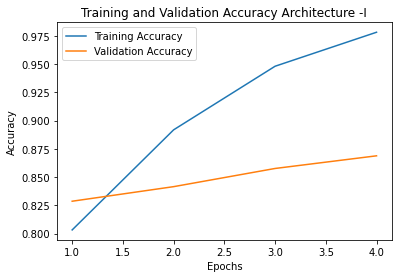
\includegraphics[width=0.9\textwidth]{Arch1Losses.png}
    \caption{Graph for best performance for first architecture}
    \label{fig:LossArch1}
\end{figure}
\begin{figure}[H]
    \centering
    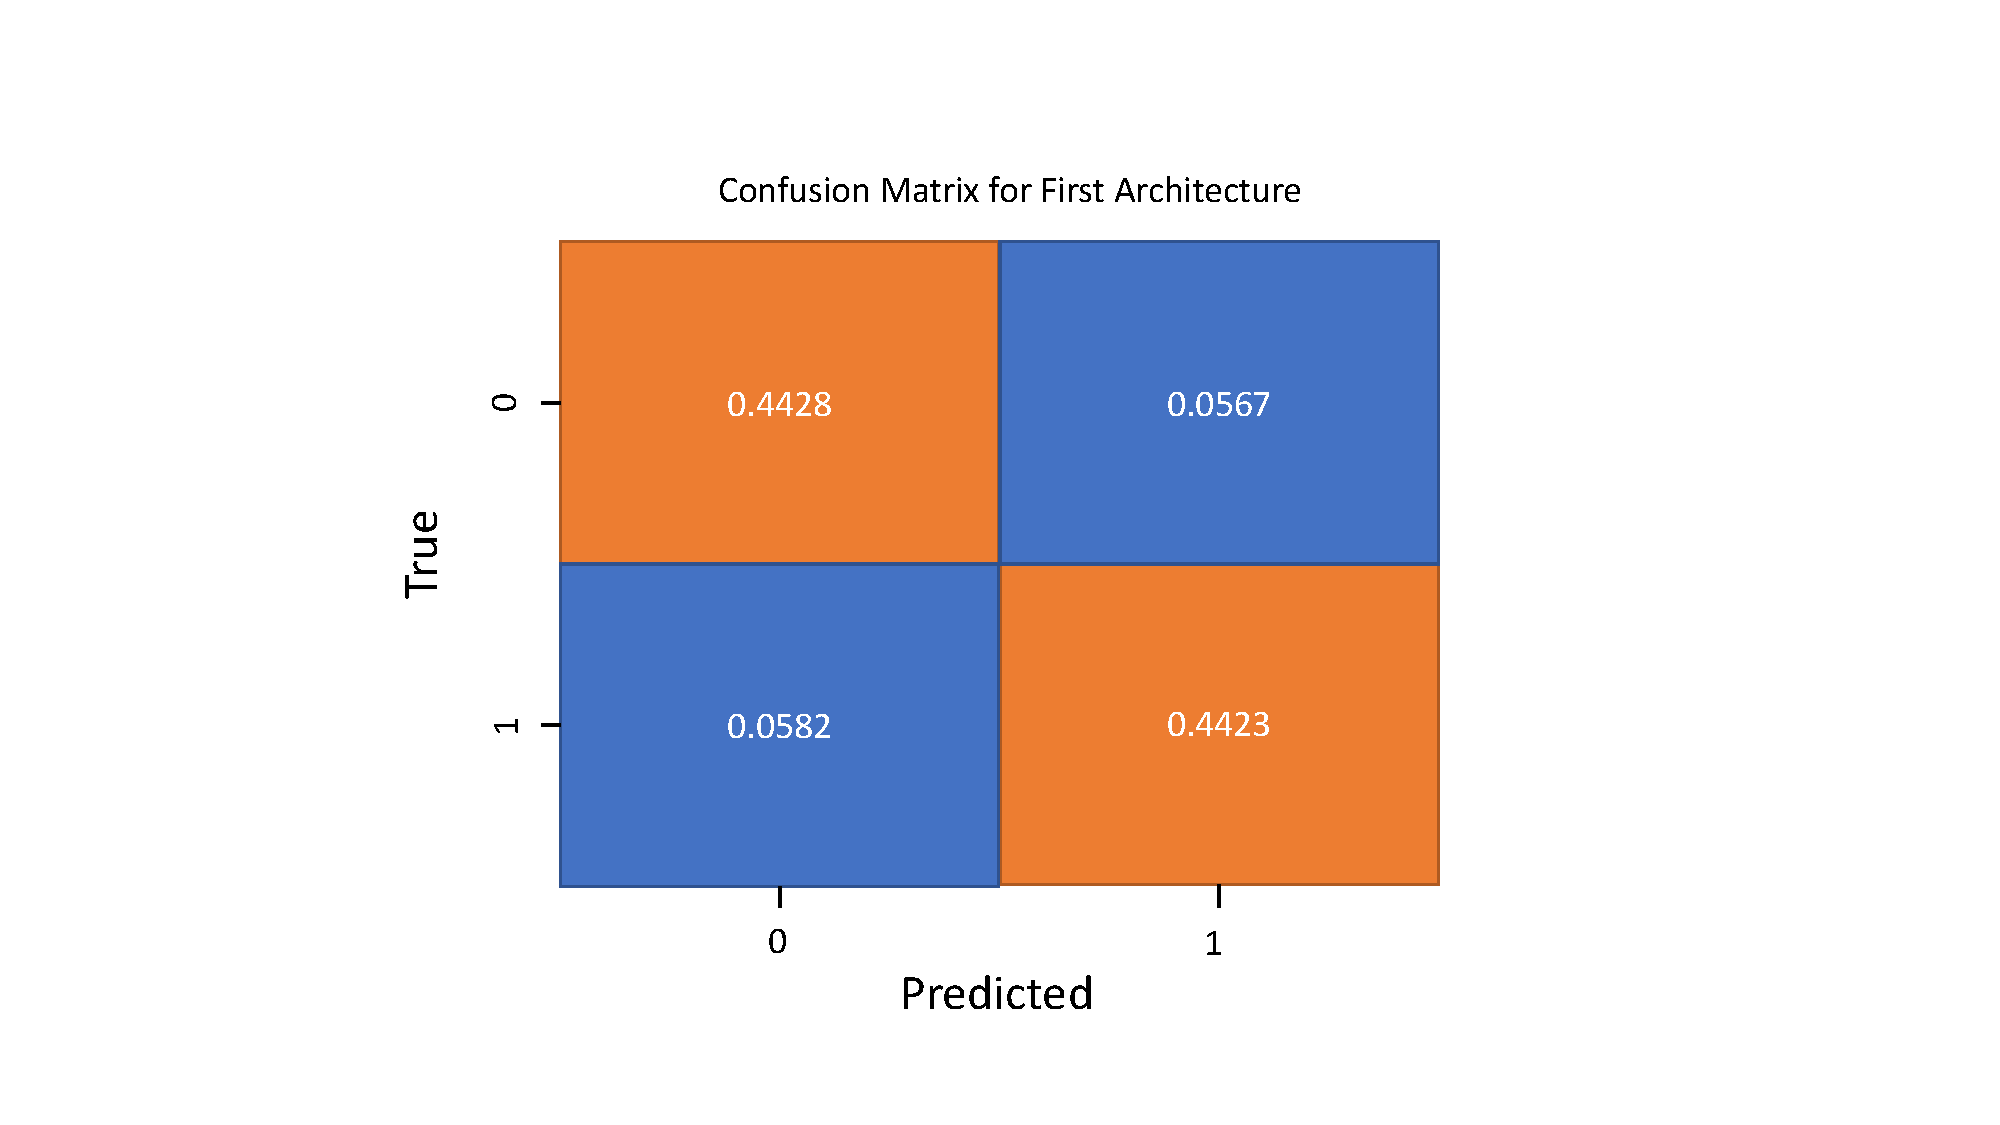
\includegraphics[width=\textwidth]{Confusion_matrix_First_Arch.pdf}
    \caption{Confusion Matrix for best performance for first architecture}
    \label{fig:Conf}
\end{figure}

\subsection{Model Architecture 2}

The table below provides a summary  of  training accuracy, validation accuracy, training loss and validation loss for the second model architecture with details of different hyperparameters used for those observations. We tried six trial runs in total for the second architecture with different sets of hyperparameters. On comparison between the results obtained from different models for the this architecture, we observed highest validation accuracy of 86.9\% and lowest validation loss of 0.30. We achieved the higher validation accuracy and minimum loss using the Sr. No. 1  hyperparameters values as mentioned in the following table. We achieved minimum values of validation accuracy and highest validation loss using the hyperparameters mentioned at Sr. No. 3 mentioned in the following table for architecture 2.\newline
\newline
\begin{tabular}[H]{ |p{0.4cm}|p{1cm}|p{1.3cm}|p{1.15cm}|p{1.25cm}|p{1.25cm}|p{1.3cm}|p{1.34cm}|p{1.45cm}|p{1.45cm}|}
\hline
 \multicolumn{10}{|c|}{Table 4:Summary of training and validation accuracy,losses for Model architecture 2} \\
 \hline
 Sr. No. & Epochs & LSTM cell & Dropout & Learning rate & Dense layers & Training loss & Training accuracy & Validation loss & Validation accuracy\\
 \hline
 1 & 4 & (128,64) & 0.2 & 0.001 & (128,256) & 0.1822 & 0.9312 & 0.307 & 0.8688 \\ 
 2 & 4 & (128,14) & 0.5 & 0.001 & (128,256) & 0.0.342 & 0.9897 & 0.59 & 0.854 \\
 3 & 3 & (128,64) & 0.3 & 0.0001 & (128,256) & 0.7066 & 0.5039 & 0.5071 & 0.5 \\
 4 & 5 & (28,14) & 0.2 & 0.001 & (128,64) & 0.0207 & 0.9928 & 0.61 & 0.853 \\
 5 & 5 & (512,256) & 0.2 & 0.0001 & (128,64) & 0.0083 & 0.997 & 0.307 & 0.8337 \\
 6 & 2 & (512,256) & 0.2 & 0.001 & (128,64) & 0.1586 & 0.9381 & 0.34 & 0.864 \\
 \hline
\end{tabular}


\begin{figure}[H]
    \centering
    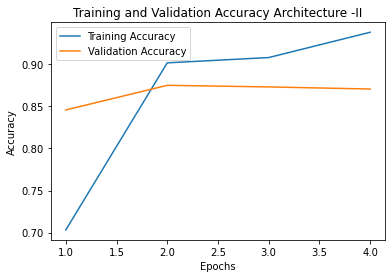
\includegraphics[width=0.9\textwidth]{MicrosoftTeams-image.png}
    \caption{Graph for best performance for second architecture}
    \label{fig:LossArch2}
\end{figure}

\begin{figure}[H]
    \centering
    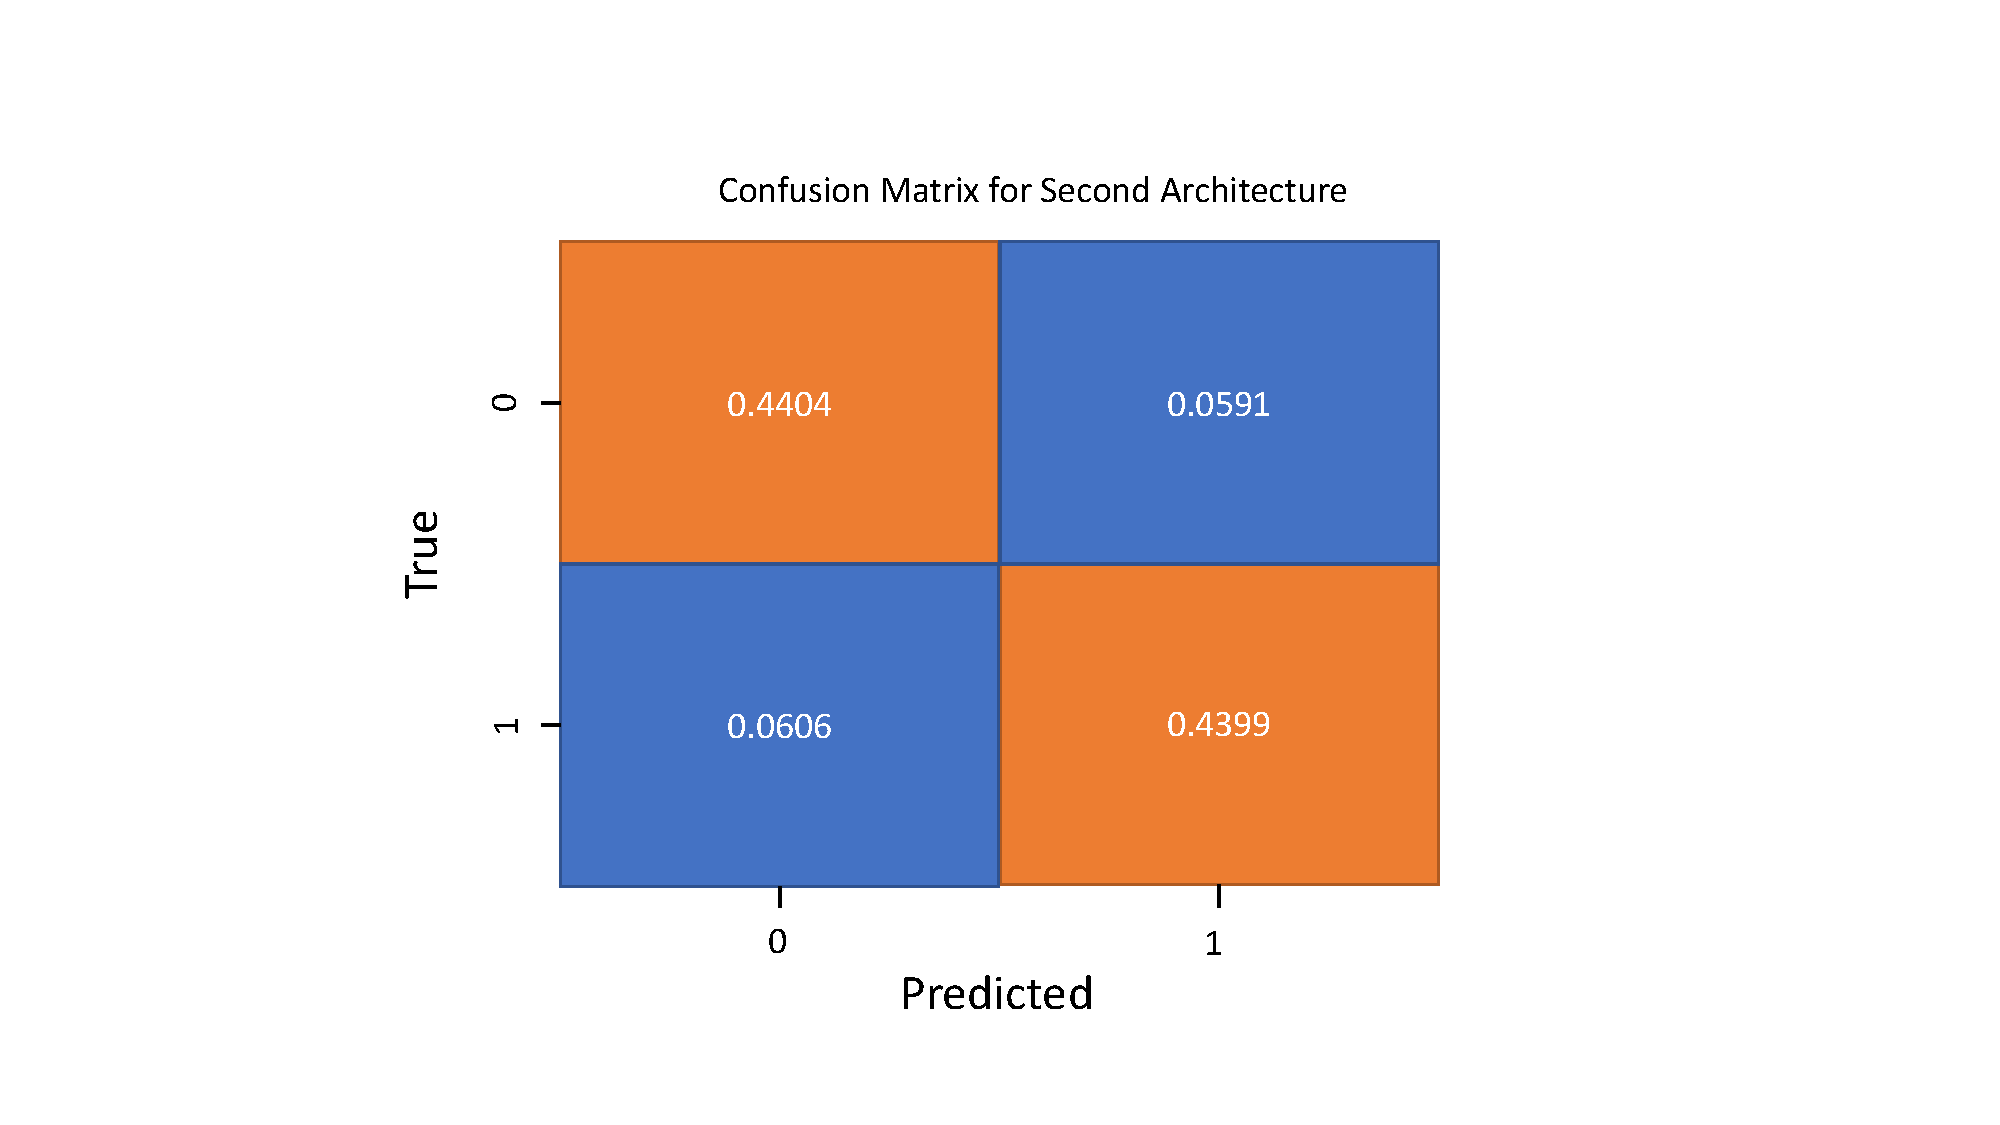
\includegraphics[width=\textwidth]{Confusion_matrix_second_arch'.pdf}
    \caption{Confusion Matrix for best performance for Second architecture}
    \label{fig:Conf2}
\end{figure}

\section{Discussion}

For this homework assignment, we started with a simple model architecture based on LSTM cells and attention mechanism. We tried two different architectures with tuning of hyper-parameters to reach higher accuracy. We began with 4 epochs and number of folds was also set to 4 . We got validation accuracy around 84.3\% with training accuracy 98.5\%.  There was a significant difference between training and validation performance. This made us to think about  applying regularisation techniques. We started with an addition of L1 regularisation but the  performance decreased steeply to  50\%. Then, we switched to L2 regularisation that did give us a better result but not much improvement over previous trials. We got the best validation accuracy of 87.07\% with a 95\% confidence interval of (0.1221, 0.1369) for the first architecture. To obtain this, we decreased the number of epochs to 4 while keeping the same number of folds without using any regularisation. Similarly, for second model architecture, we proposed a deeper model with the addition of more convolution and pooling layers along with two dense and drop out layers. Initially, we set dropout to 30\% with 128 and 256 neurons in two dense layers having learning rate of 0.0001. We ran this configuration for 3 epochs but it performed very poor and landed validation accuracy of mere 50\%. After testing out different variations, the highest validation accuracy we were able to achieve with second architecture was 86.88\%.  It was seen that most of these models were not very significantly different from each other when it comes to performance. But, adding dropout layers did help with overfitting in the second architecture as there was not a mojor difference between training (93.12\%) and validation (86.88\%) accuracies with a 95\% confidence interval of (0.1206, 0.1348). An important insight gained from this project is the intuition behind tuning hyper-parameters and predict their affect on model's performance.







\section{Conclusions}

For this homework assignment, we managed to create an LSTM based architecture that achieved a good validation accuracy on IMDB dataset. The best model architecture gave accuracy of 87.08\% on the unseen test data. This helped us to learn the benefit of sequential hyper-parameter tuning for making better-performing model architectures. Addition of dropout layers reduced the amount of overfitting in the second architecture. This assignment also helped us to develop an intuition about tuning the hyper-parameters sequentially and made us learn how that will affect model's performance. We believe that performance can still be improved by using architectures that make use of bidirectional GRU that can tackle the problem of vanishing gradients as we encountered in the second architecture. Also, the use of pre-trained model weights available for similar sentiment analysis tasks can be used as a starting point and then, fine tuning the model can result in better performance.

\begin{table}[H]
    \caption{Contributions by team member for this assignment.}
    \centering
    \begin{tabular}{|c|c|} \hline
    {\bf Team Member}     &  {\bf Contribution}  \\ \hline
    Shiva Paudel     & Experimental results and Experimental setup   \\
    Kantilata Thapa   & Introduction,problem description and model architecture 1 \\
    Shubham Bery    & Abstract,Discussion and conclusion \\
    Puranjit Singh     & Approaches and  Model architcture 2  \\\hline
    \end{tabular}
    \label{tab:contribution}
\end{table}

\bibliographystyle{plainurl}
\bibliography{main}

\end{document}
